\documentclass[11pt,titlepage]{article}
\usepackage[a4paper,margin=1in]{geometry}
\usepackage[T1]{fontenc}
\usepackage[english]{babel}
\usepackage{lmodern,microtype,csquotes}
\usepackage{amsmath,booktabs,tabularx,array,multicol}
\usepackage{tikz}
\usetikzlibrary{arrows.meta,positioning}
\usepackage{xurl}
\usepackage[backend=biber,style=apa]{biblatex}
\addbibresource{references.bib}
\usepackage[hidelinks]{hyperref}

\setlength{\emergencystretch}{3em}
\setlength{\parindent}{1em}
\setlength{\parskip}{0.3\baselineskip}
\setlength{\columnsep}{0.3in}
\setcounter{secnumdepth}{0}
\setcounter{tocdepth}{2}
\raggedbottom
\newcolumntype{Y}{>{\raggedright\arraybackslash}X}

\title{Generative AI in Duolingo:\\[0.5em]
\large Feedback, Conversation Practice, and Learner Engagement}
\author{Author One \\ Student number: [to be supplied]
\and Author Two \\ Student number: [to be supplied]}
\date{Applied AI --- Research Paper\\Evidence reviewed through September 11, 2026}

\begin{document}
\maketitle
\pagenumbering{roman}
\begin{multicols}{2}
\section*{Abstract}
This paper examines what existing research establishes about the effects of Duolingo's generative-AI feedback and conversation features on learners' confidence and engagement. A focused, AI-assisted documentary review compares Explain My Answer, Roleplay, and Video Call with conventional app practice, then appraises direct Duolingo evidence alongside transferable research. Confidence is distinguished from tested proficiency, and engagement is separated into behavioral, emotional, and cognitive dimensions. Direct findings are mixed and conditional: an uncontrolled study reports self-efficacy improvements among selected users, while a company speaking report finds stable willingness to communicate and neutral confidence perceptions despite a performance benefit. A later company summary reports positive confidence findings in another population but supplies insufficient detail for full appraisal. Platform-reported speaking volume provides participation evidence, not proof of learning or voluntary persistence. Wider studies show that interface design, teacher support, language proficiency, and feedback literacy can influence outcomes, but do not validate Duolingo automatically. The synthesis identifies limitations involving feedback correctness, conversational support, speech recognition, selection, outcome measurement, and transfer. The review concludes that these features expand opportunities for supported practice, while durable improvements in confidence and meaningful engagement remain insufficiently established across versions and learner groups. A feature-level evaluation framework specifies how stronger claims could be tested.

\noindent\textbf{Keywords:} Duolingo; generative AI; corrective feedback; conversation practice; self-efficacy; learner engagement.
\end{multicols}
\clearpage
\tableofcontents
\clearpage
\pagenumbering{arabic}
\twocolumn

\section{Introduction}
\label{sec:introduction}
\subsection{The Problem: More Interaction, but What Benefit?}
Duolingo's generative features create a concrete applied-AI question: does making practice more responsive improve how learners experience and engage with it? Duolingo Max introduced explanations and roleplay in March 2023, while Video Call was announced in September 2024 \parencite{maxLaunch,duocon2024}. These developments extend an established application rather than replace a previously non-adaptive learning environment. The earlier teaching-method account already emphasized structured activity, personalization, and sustained participation \parencite{freeman2023}.

The relevant distinction is between selecting an existing task and generating language in response to a learner. An adaptive system can choose an appropriately difficult exercise without composing its wording; a generative system can formulate a contextual explanation or a conversational reply. Duolingo's production account distinguishes adaptive exercise selection from language-model generation \parencite{contentProduction}. This paper concentrates on generation during learner interaction, not the separate question of automating course authorship.

The educational significance cannot be determined from responsiveness alone. A conversational reply may encourage another attempt without correcting an error. An explanation may feel reassuring without improving understanding. Conversely, accurate feedback may initially reduce confidence by revealing a gap. These possibilities motivate an outcome-specific review rather than an assumption that a more conversational interface necessarily provides a better learning experience.

\subsection{Confidence and Engagement as Distinct Outcomes}
Here, \emph{confidence} is an umbrella term for perceived ability; \emph{self-efficacy} refers more specifically to beliefs about performing a particular language task. Willingness to communicate concerns readiness to enter an exchange and is treated as related, but not identical. None is a proficiency score. The Duolingo self-efficacy study makes task-specific capability beliefs central to its investigation \parencite{kittredge2025self}.

Engagement is likewise more than the number of app visits. Following the multidimensional approach used by \textcite{loEngagement2024}, this review distinguishes behavioral participation, emotional involvement, and cognitive investment. The distinction allows an activity to be frequent or enjoyable without assuming that the learner evaluates feedback or develops independent control. Motivation, anxiety, and autonomy are discussed only where they explain these focal outcomes, not as additional comprehensive research topics.

This scope matters for learners and educators deciding what an AI-supported activity can reasonably provide. It also matters for developers choosing evaluation targets: confidence, participation, and learning should be reported in their own terms rather than used interchangeably.

\subsection{Research Question and Objective}
The objective is to describe the selected features, appraise evidence about confidence and engagement, and identify the design and research limitations that constrain interpretation.

\noindent\textbf{Main research question}

What does existing research show about the effects of Duolingo's generative-AI feedback and conversation features on learners' confidence and engagement?

\noindent\textbf{Sub-questions}
\begin{enumerate}
    \item How do Duolingo's generative-AI feedback and conversation features introduced since 2023 differ from its conventional exercises and feedback?
    \item What Duolingo-specific evidence exists that these features affect learners' confidence and engagement, and how does it compare with findings from wider generative-AI language-learning research?
    \item What limitations in feature design and research evidence constrain conclusions about these effects?
\end{enumerate}

\subsection{Scope and Reading Guide}
The review covers Explain My Answer, Roleplay, and Video Call with Lily and Falstaff. Conventional lessons provide the comparison. Course generation, catalog expansion, and commercial priorities appear only as limited Discussion context. Other Duolingo subjects and the Duolingo English Test are excluded as separate products. Speaking performance is included to assess whether perceived and demonstrated capability align, not to conduct a comprehensive efficacy review. The \nameref{sec:method} section explains selection and appraisal; \nameref{sec:results} addresses the three questions; \nameref{sec:conclusion-discussion} provides the overall answer and recommendations.

\clearpage
\section{Method}
\label{sec:method}
\subsection{Design, Population, and Selection}
This is a focused, AI-assisted documentary review. It is not preregistered systematic screening, an experiment, or a product audit. The population of interest comprises public documentation and research relevant to the selected features, learner confidence, and engagement. The sample consists of documents. No learners were recruited, accounts tested, internal code inspected, or model outputs independently scored.

The review uses the supplied 222-record research inventory and the earlier source audit as discovery resources, then extends targeted retrieval through September 11, 2026. Inventory entries contain metadata and annotations, not participant-level data or 222 fully inspected studies. Retrieval used exact titles, DOIs, named features, outcome terms, and publisher, author-hosted, company, or institutional versions. Additional searches combined Duolingo, Roleplay, and Video Call with confidence, engagement, and self-efficacy, and sought comparative studies of generative conversation, feedback use, and teacher support. A search and decision record accompanies the paper in \texttt{research/focused-review-audit.md}.

Inclusion required an identifiable source and a relevant inspectable passage. Three evidence classes were retained: product documentation establishing reported functionality; direct or adjacent Duolingo research; and external research addressing a comparable mechanism or outcome. Production-only studies, unrelated products, anecdotal forum posts, and sources lacking sufficient relevant text were not used to estimate feature effects. Exclusion from this focused synthesis does not establish that a source is invalid or irrelevant to other questions.

\subsection{Extraction and Critical Appraisal}
For primary learner studies, extraction records population, feature exposure, duration, comparison, outcome instrument, finding, analysis population, provenance, and access completeness. Exposure is classified as \emph{confirmed generative feature}, \emph{general Duolingo use}, or \emph{uncertain}. A publication date after 2023, an AI label, or comparison with ChatGPT does not establish that the Duolingo condition used generation. \texttt{research/focused-evidence.csv} provides the study-level extraction matrix.

Appraisal evaluates four questions: does the intervention match the claim; does the comparison support attribution; does the measure represent the stated outcome; and does the sample support transfer? Company affiliation, peer review, and sample size are considered separately. Studies are not assigned a numerical quality score. Performance results are not renamed confidence, and app activity is not equated with cognitive engagement. Both positive and non-significant findings are retained.

Where possible, original methods, results, participant-flow figures, and limitations were inspected. Abstract-only or indexed-passage access is explicitly identified. For the self-efficacy paper, the original published PDF was checked against its flow diagrams and regression tables. The Japanese-English Video Call report remained accessible through indexed original-report passages rather than a complete downloaded copy. Its post-test and post-survey populations are therefore distinguished without a new analysis of participant records. Descriptions of unavailable procedures are not reconstructed.

\subsection{Synthesis and Evidence Boundaries}
Results follow \emph{feature comparison, outcome-specific evidence, and limitations}. Tables connect claims to exposure and measurement; the figure is an analytical framework, not a discovered production architecture or estimated causal model. Quantitative values are reported from publications, not recomputed as a meta-analysis. Review samples are not added together because underlying studies can overlap. Broad AI reviews are not automatically classified as evidence about generative systems.

The evidence cutoff is September 11, 2026, not a single product release. Announcement, rollout, study, and publication dates remain separate. Live pages may describe newer behavior than a historical study evaluated. Terminology and reference dates follow the inspected publication version, with online and issue dates distinguished where relevant. Historical audits remain available, but this focused audit supersedes their scope and corrects the earlier draft's mistaken self-efficacy cohort split.

This method supports a critical account of what the available evidence establishes, not an exhaustive count of all research or a causal estimate for the entire user population. Author checking and independent peer review remain necessary safeguards, particularly for mutable documents, incomplete access, and AI-assisted extraction.

\clearpage
\section{Results}
\label{sec:results}
\label{sec:results-start}

\subsection{RQ1: Features Compared with Conventional Practice}
\label{sec:rq1}
\subsubsection{An Adaptive, Gamified Baseline}
The comparison is not between AI and no AI. \textcite{shortt2023} review Duolingo research covering 2012 to early 2020, establishing a historical literature on gamification before Max. \textcite{liBonk2025}, first published online in 2023 after submission in 2022, describe ten users' self-directed learning with the app and other resources. These sources show why personalization, learner choice, and motivational design cannot be credited entirely to later generative features. They do not establish one uniform historical experience across courses or users.

The functional baseline is a learner completing a structured task, receiving a correctness judgement or predefined support, and progressing through a designed sequence. The feature comparison asks what additional action becomes possible: requesting a contextual explanation, contributing an unanticipated response, asking for clarification, or reviewing a conversation. It does not assume that the earlier application lacked every form of speaking practice or explanation. The relevant difference is the responsiveness and scope of the interaction, not the presence of a microphone or a feedback message alone.

Table~\ref{tab:features} separates reported capabilities from the hypotheses they motivate. The final column is deliberately phrased as an evaluation question: product documentation can establish that a function is offered without establishing its effect on confidence or engagement.

\begin{table*}[t]
\centering
\small
\caption{Feature comparison and evaluation targets. Capabilities are developer-reported; outcome questions are this review's analytical interpretation.}
\label{tab:features}
\begin{tabularx}{\textwidth}{@{}>{\raggedright\arraybackslash}p{0.18\textwidth}YYY@{}}
\toprule
Feature & Reported difference from conventional practice & Principal learner action & Outcome question \\
\midrule
Explain My Answer \parencite{explainFree} & Contextual explanation beyond correctness feedback & Request and interpret assistance & Does reassurance accompany understanding and independent reuse? \\
Roleplay \parencite{roleplayDesign} & Generated dialogue within a designed scenario & Formulate, clarify, and respond & Does supported participation extend beyond following suggestions? \\
Lily Video Call \parencite{henry2025} & Spoken exchange with contextual and dialogue-stage controls & Maintain and redirect conversation & Does greater speaking activity coincide with confidence and meaningful contribution? \\
Falstaff Video Call \parencite{falstaff} & Guided conversation with phrases, translations, and feedback & Practise with graduated assistance & Does support enable subsequent production without the same prompts? \\
\bottomrule
\end{tabularx}
\end{table*}

\subsubsection{The Timeline Defines Which Claims Are Possible}
The March 14, 2023 Max announcement concerns Explain My Answer and Roleplay, historically attributed to GPT-4 \parencite{maxLaunch}. Video Call was announced on September 24, 2024 \parencite{duocon2024}. Its January 16, 2025 Android expansion is a later rollout event, not its original launch. That release also describes transcript review and incoming calls as iOS enhancements, with later Android availability planned \parencite{android2025}. These distinctions prevent attributing a 2023 intervention to a feature introduced subsequently.

Access also changes independently of model capability. A December 29, 2025 report identified January 1, 2026 as the announced start of free Explain My Answer access; the company page qualifies course coverage \parencite{explainAccess2025,explainFree}. In its May 4, 2026 filing, Duolingo reported beginning expansion of Video Call to Super subscribers \parencite{shareholderQ12026}. Neither statement proves simultaneous access for every account. A study's subscription tier, device, course, and date remain part of its intervention definition.

\subsubsection{Explanation: From an Answer to a Reason}
Explain My Answer provides requested explanations related to a response and the language pattern involved. The company describes attention to the learner's error and language background, including examples of how grammar can differ between languages \parencite{explainFree}. Its potential contribution is therefore not just additional text. It can connect a local mistake with a reason the learner can use on another occasion.

This creates an important distinction between delivery and uptake. For example, a learner might read a correct explanation of article agreement, select the corrected answer, and still fail to apply the rule to a new noun. That hypothetical sequence would demonstrate access and immediate task completion, but not necessarily understanding. Conversely, declining an explanation after recognizing a simple typing error could be an appropriate choice rather than disengagement. Meaningful use cannot be inferred from clicks alone.

The historical feature and its current free implementation should also not be treated as experimentally identical. A change in access can alter the users who encounter an explanation, while changes in presentation can alter how much they read or request. The study question is whether a specific form of assistance helps a defined user group, not whether the feature name remains unchanged. This is an interpretive boundary, not evidence that later versions are better or worse.

\subsubsection{Roleplay: Generative but Still Structured}
Duolingo describes Roleplay as a sequence of specialized prompts rather than one unrestricted chatbot instruction. The prompts receive scenario, character, learning-objective, and proficiency-related context, while application logic manages stages of the exchange \parencite{roleplayDesign}. The mechanism reduces the need for learners to design their own practice prompts. It also means that observed outcomes belong to a combined instructional design, not a language model operating alone.

A scenario can provide a reason to communicate, but completing it does not reveal how independently the learner acted. A user who selects suggested phrases and a user who negotiates an unexpected misunderstanding may reach the same endpoint through different cognitive demands. For evaluation, the important contrast is not simply successful versus unsuccessful completion. It includes whether the learner generates contributions, recognizes mismatches, and adjusts a message to achieve the conversational goal.

\subsubsection{Spoken Conversation: Continuity and Guidance}
The Lily account describes staged openings, contextual questions, continued interaction, and managed endings. It also documents transcript-derived facts supplied as context for subsequent calls and checks intended to support topic redirection \parencite{henry2025}. These mechanisms explain how an exchange can respond to a learner without requiring an unrestricted or continuously retrained model. They do not establish that personalization is always accurate or that every learner experiences it as useful.

Falstaff is described differently: a guided partner offering level-related questions, suggested phrases, translations, and feedback in the learner's own language. Its live page describes an expansion across proficiency levels, whereas the beginner study concerns a narrower population \parencite{falstaff}. Guidance and open conversation are consequently different instructional conditions, not interchangeable instances of ``AI speaking.''

The comparison is educationally important. Assistance may lower the threshold for making a first contribution, while fewer prompts may demand more retrieval and conversational initiative. Neither condition is inherently preferable for every learner. A useful evaluation would identify when support enables participation and when the same support conceals dependence. This review treats that relationship as a testable design question, not a documented effect of one character's personality.

\subsubsection{What RQ1 Establishes}
The features expand opportunities for explanation and responsive practice beyond a constrained exercise. However, their educational unit is the complete interaction: task, model instructions, assistance, speech interface, and opportunities for review. Identifying that unit is necessary before comparing outcomes. An experiment on a general chatbot, or an earlier feature version, cannot establish the effect of every element simply because generation is involved.

The baseline also remains relevant after adoption. Learners continue to complete ordinary lessons while using optional generative activities. Outcomes observed during this mixed exposure cannot be attributed wholly to the new features without a comparison that addresses the conventional practice. RQ2 therefore distinguishes what users encountered, what was measured, and which alternative explanation remains possible.

\subsection{RQ2: Confidence and Engagement Evidence}
\label{sec:rq2}
\subsubsection{A Claim-by-Claim Evidence Map}
Table~\ref{tab:direct} organizes the closest Duolingo evidence by claim rather than combining all positive outcomes. A source can be direct about feature exposure yet weak for causal attribution. Likewise, externally authored research can be independent without evaluating the relevant feature. The table is not a count of independent replications: summaries and underlying reports may describe overlapping studies.

\begin{table*}[t]
\centering
\small
\caption{Direct evidence mapped to outcomes. C = confidence or related self-report; B = behavioral engagement; P = language performance. These are outcome labels, not quality scores.}
\label{tab:direct}
\begin{tabularx}{\textwidth}{@{}>{\raggedright\arraybackslash}p{0.23\textwidth}YYY@{}}
\toprule
Source & Exposure and outcome & Evidential contribution & Main boundary \\
\midrule
\textcite{kittredge2025self} & Roleplay/Explain My Answer; C & Task-specific self-report & Selected users; uncontrolled \\
\textcite{kittredge2025video} & Lily; Japanese-English; C, P & Outcomes can diverge & Different analysis populations; adherence exclusions \\
\textcite{videoResearch} & Lily; English-Spanish; C, P & Later positive confidence report & Company summary; methods incomplete \\
\textcite{falstaffResearch} & Guided calls; beginner French/Spanish; P & Practised phrase production & Not a direct confidence measure \\
\textcite{shareholderQ12026} & Video Call; B & Aggregate speaking-volume indicator & No controlled engagement evaluation \\
\textcite{harrison2025} & Video Call and other voice tools & External affordance review & Not a learner-outcome trial; abstract-only access \\
\bottomrule
\end{tabularx}
\end{table*}

The comparison supports three separate questions: do learners feel more capable; do they participate differently; and does that participation involve understanding? A speaking test can inform the relationship between confidence and capability, but cannot substitute for a confidence measure. Similarly, a survey of perceived usefulness is not a record of voluntary persistence. This separation prevents a broad claim from appearing stronger merely because it combines several narrower, non-equivalent findings.

\subsubsection{Self-Efficacy: Positive but Selective Findings}
\textcite{kittredge2025self} collected data between August 30 and November 17, 2023. Final analyses included 153 existing subscribers and 232 newly granted-access learners, totaling 385. Across one-month exposure to Roleplay and Explain My Answer, the reported significant change concerned one of seven self-efficacy items in the existing-user cohort and six in the new-access cohort. There was no non-feature control. Seven of seventeen collected items were selected for analysis, six-point responses were dichotomized, and multiple comparisons were adjusted. Feature-use counts did not significantly predict post-survey self-efficacy. Usage requirements selected adherent participants; all authors were affiliated with Duolingo.

These are findings about perceived capability, not a proficiency estimate. An existing-user cohort is not an untreated control, and differences between paid and complimentary access do not isolate novelty experimentally. Both groups also continued ordinary practice. The analysis therefore supports a bounded statement about selected users' responses, not a general claim that either feature causes confidence gains or that additional use necessarily increases them.

The lack of a significant usage association does not establish that practice is irrelevant. A selected sample, a restricted exposure range, and coarse outcome coding can make relationships difficult to detect. Conversely, those possibilities cannot be used to assert an effect that was not demonstrated. The correct evidential position is to retain the reported result while treating causal explanation as unresolved.

\subsubsection{Lily: Performance and Confidence Do Not Necessarily Align}
The June 24, 2025 company report on Japanese learners of English followed 658 learners into two 30-day conditions. Post-test analysis included 567 and post-survey analysis 558. It reports a small performance advantage for regular Lily-call users, but willingness to communicate remained stable and confidence perceptions after using the feature were neutral. The call condition required at least two calls daily; exclusions were more frequent there. Average words per call predicted speaking post-test scores, an association rather than a randomized dose effect \parencite{kittredge2025video}. Relevant original-report passages, including participant flow and conclusions, were inspected through indexing.

This result is particularly important for the narrowed question. More successful test performance does not guarantee a corresponding subjective change. Equally, stable willingness to communicate is not proof that an activity has no educational value. The report's confidence perception and repeated willingness measure should not be merged into one pre/post confidence score. They answer different questions, and neutral responses should not disappear when the overall feature is described as promising.

A later company summary describes English speakers learning early-intermediate Spanish who showed greater speaking improvement and reported higher confidence with Lily than with regular lessons. It does not supply sufficient sample, assignment, instrument, or effect-size details for a full appraisal \parencite{videoResearch}. The contrast with the Japanese-English report could reflect population, version, instrument, or study-design differences. Without matched measures, it is neither a direct contradiction nor a validated explanation of who benefits most.

\subsubsection{Guided Calls and Observable Participation}
The Falstaff summary compares beginner French and Spanish learners who had completed equivalent course units, with or without guided calls. The test required spoken translations and included phrases practised during the calls. Call users scored higher, but the summary lacks sufficient assignment and sample details for strong causal conclusions \parencite{falstaffResearch}. This is evidence about target phrase production, not direct evidence of confidence or freely initiated conversation.

Observable participation provides another perspective. Duolingo's May 4, 2026 filing reports that the average number of words spoken per user in Video Call more than doubled over the preceding year \parencite{shareholderQ12026}. This is a feature-specific behavioral indicator, but the passage does not provide a fixed-version comparison, user-composition adjustment, or a validated cognitive-engagement measure. More words could reflect more calls, longer turns, interface changes, or a different user population. The statistic cannot identify which explanation applies.

Consequently, the direct behavioral record is more informative than a claim that no engagement evidence exists, but less informative than a controlled evaluation of meaningful engagement. A denominator matters: words per active caller, words per eligible user, and words per call describe different populations. A change among continuing callers may coexist with substantial abandonment among those who tried the feature. Aggregates need participant flow and task context to become evidence about the broader experience.

\subsubsection{External and Feature-Uncertain Duolingo Studies}
\textcite{harrison2025} explicitly reviews Video Call alongside other conversational tools. The accessible SSRN abstract supports classification as a technology review, not an experiment measuring learner change. Independence is valuable for perspective but cannot compensate for a different research design. Detailed judgments from the inaccessible full text are not reconstructed.

\textcite{ouyang2024} examine an eighty-learner Duolingo-supported EFL intervention involving self-reported willingness to communicate and engagement. The inspected methods do not establish the named generative features. Likewise, the accessible publisher material for \textcite{xu2025} identifies Duolingo versus ChatGPT and relevant psychological outcomes without adequately establishing the Duolingo feature version. The former is general-app evidence and the latter feature-uncertain. Neither is used to estimate a Max-specific effect.

These distinctions are substantive, not simply restrictive. A general-app intervention can show what conventional or mixed practice might achieve, helping define a comparator for a generative-feature study. It can also identify measurement approaches worth reusing. What it cannot do is answer a technology-specific question when exposure is undocumented. A comparison with ChatGPT establishes a generative condition on one side, not necessarily on both.

\subsubsection{Comparable Speaking Studies: Benefits Depend on Design}
\textcite{wangConversation2024} compare three groups of 33 Chinese undergraduates: teacher/peer interaction, text-and-voice chatbot interaction, and an avatar-based generative condition. The avatar condition improved willingness to communicate and self-perceived competence and reduced speaking anxiety relative to the control, without a significant between-group speaking-performance advantage. The methods describe convenience-selected classes, not an individually randomized test of Duolingo. The reported intervention combines interface, dialogue, and instructional components; it does not isolate an avatar effect alone.

This is a useful counterpoint to the Japanese-English call report: favorable affective outcomes can occur without a demonstrated performance advantage, just as a performance advantage can occur without more favorable confidence perceptions. The comparison does not estimate either relationship causally across studies. Its purpose is to show why the outcomes should be measured together rather than assumed to move in parallel.

\textcite{celik2025} report an eight-week ChatGPT-supported intervention with 44 university learners in Iraq and higher speaking self-efficacy in the experimental group. Close reading qualifies the abstract: the methods describe convenience sampling, while the intervention adds home practice, training, and additional lecturer-supported speaking. It is therefore not a clean test of replacing classroom speaking with an otherwise equivalent chatbot activity. The study supports investigating supported practice, not attributing the entire difference to generation or transferring its magnitude to Duolingo.

\subsubsection{Engagement: Emotion, Activity, and Understanding}
\textcite{yan2024} examine four Chinese university writers over a five-week ChatGPT-feedback project using prompts, revisions, journals, and interviews. Engagement differed with language proficiency and technological competence; favorable reactions did not ensure effective feedback use. Only four of fourteen volunteers supplied complete data. This small, selected case study cannot estimate average effects, but its interaction-level evidence shows why cognitive engagement needs closer observation than a satisfaction questionnaire.

An application-designed prompt can reduce the burden of asking for feedback, but cannot remove the learner's need to interpret it. The transferable mechanism is the difference between receiving, accepting, and understanding assistance. Extended academic writing is not a Duolingo sentence exercise; consequently, the study informs what to inspect rather than how frequently a problem occurs in Explain My Answer. Transferring a measurement idea is more defensible than transferring an unmeasured product-level effect.

Teacher support is another boundary. \textcite{liTeacher2026} compare sixty learners in generative-chatbot language learning, thirty with teacher presence and thirty without. The teacher-presence group reported higher emotional and agentic engagement, but not significantly different behavioral or cognitive engagement. This establishes a distinction within the investigated setting, not a universal teacher effect. It also illustrates why classroom-supported findings cannot be assumed to reproduce in an unsupervised consumer app.

\subsubsection{What Wider Syntheses Add---and Cannot Add}
\textcite{loEngagement2024} synthesize 72 empirical ChatGPT studies from its first year. Behavioral evidence is comparatively concentrated on using the tool; emotional findings are mixed, and cognitive-engagement evidence is broad but weak. The review extends beyond language learning. Its main contribution here is therefore the outcome framework and caution about uneven evidence, not a Duolingo effect estimate.

Language-learning meta-analyses provide wider quantitative context. \textcite{liMeta2025} report 41 studies, 3,515 participants, and a pooled effect of 0.576 (95\% CI 0.385--0.768). The accessible publisher abstract supports this aggregate result, not a detailed reappraisal of every included study. \textcite{saarela2026} synthesize 51 studies and report positive aggregate results alongside substantial heterogeneity ($I^2=98.4\%$ in the reported overall analysis) and significant small-study effects. Their sensitivity checks retained the main conclusions; heterogeneity is therefore a qualification, not a reason to discard all positive findings.

\textcite{liTask2026} review 25 task-based studies involving 2,431 participants. Their analysis highlights AI literacy, task planning, and assessment arrangements as potential moderators. This connects benefits to instruction rather than to an undifferentiated chatbot label. Across these syntheses, pooled achievement or affective--cognitive outcomes cannot be reinterpreted as a confidence effect for a particular feature. Review overlap and differences in comparisons also prevent adding sample totals or ranking products from their pooled estimates.

\subsubsection{Statistical Findings and Practical Meaning}
Statistical significance is not the same as a meaningful improvement in everyday practice. A change in questionnaire agreement can matter to a learner, but its practical interpretation depends on the item, starting point, and persistence of the change. A standardized pooled effect describes variation relative to a study's outcome scale; it is not a percentage increase in confidence or a predicted gain for a new Duolingo user. The reported results should therefore retain their original measure and comparison.

The same discipline applies to non-significant findings. Failure to demonstrate a difference is not evidence that two conditions are equivalent. Without sufficiently precise estimates and a justified equivalence margin, the defensible conclusion is that the studied contrast did not establish the effect, not that the feature cannot help anyone. Conversely, proposing low power or an insensitive measure cannot turn that result into positive evidence. This distinction makes the synthesis informative without either overselling benefits or interpreting uncertainty as failure.

\subsubsection{An Outcome-Specific Answer}
The evidence supports a qualified possibility of improved perceived capability, not a consistent confidence effect across features and populations. Direct participation indicators exist, but neither they nor positive perceptions establish durable cognitive engagement. External research makes the proposed mechanisms plausible and supplies stronger measurement approaches; it does not eliminate the limits of the direct Duolingo studies.

The remaining uncertainty is consequently specific: whether defined versions improve task-matched confidence, voluntary sustained participation, and independently demonstrated use of feedback for the users who are actually offered them. This is a more demanding claim than availability, satisfaction, or short-term activity, but a more useful one for deciding what the features contribute.

\subsection{RQ3: Design and Evidence Limitations}
\label{sec:rq3}
\subsubsection{A Mechanism Is Not an Established Causal Path}
Figure~\ref{fig:framework} represents this review's analytical model. A design can provide an opportunity, the learner can engage with it, and a later outcome can change. Each connection requires evidence. The figure does not claim that these stages form a validated sequence or that confidence is merely an intermediate step toward proficiency. Confidence and engagement remain outcomes of interest in their own right.

\begin{figure*}[t]
\centering
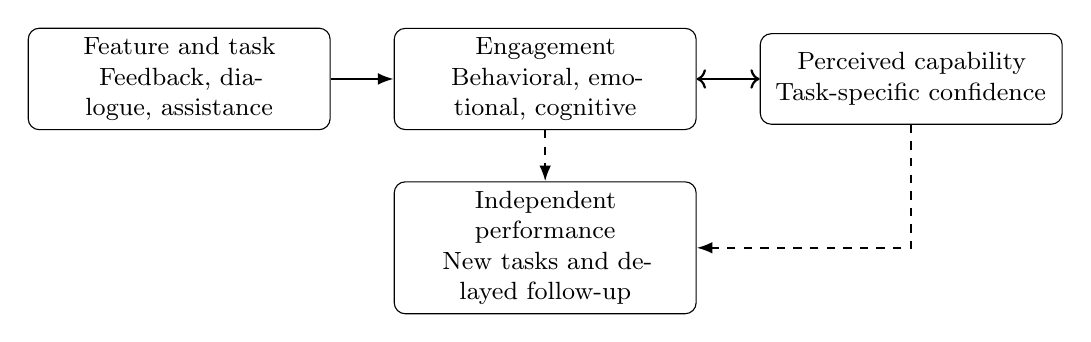
\begin{tikzpicture}[
box/.style={draw,rounded corners,align=center,text width=3.6cm,minimum height=1.15cm,font=\small},
flow/.style={-{Latex[length=2mm]},thick},
node distance=0.65cm and 0.8cm]
\node[box] (design) {Feature and task\\Feedback, dialogue, assistance};
\node[box,right=of design] (engagement) {Engagement\\Behavioral, emotional, cognitive};
\node[box,right=of engagement] (confidence) {Perceived capability\\Task-specific confidence};
\node[box,below=of engagement] (performance) {Independent performance\\New tasks and delayed follow-up};
\draw[flow] (design) -- (engagement);
\draw[flow,<->] (engagement) -- (confidence);
\draw[flow,dashed] (engagement.south) -- (performance.north);
\draw[flow,dashed] (confidence.south) |- (performance.east);
\end{tikzpicture}
\caption{Proposed relationships to evaluate, not estimated causal effects. Dashed connections identify performance checks needed to examine transfer and confidence calibration. Learner characteristics, access, and support may affect every relationship.}
\label{fig:framework}
\end{figure*}

A complete feature evaluation therefore needs more than a model benchmark. Even accurate generated language may be poorly timed, unnecessarily difficult, or irrelevant to the learner's goal. Conversely, the surrounding application can make a general model easier to use through curriculum context and assistance. The outcome belongs to that implemented combination. Without component comparisons, a successful intervention cannot reveal whether its decisive element was generation, task design, additional practice, or their interaction.

\subsubsection{Feedback Correctness and Confidence Calibration}
\textcite{luo2026} investigate how prompt sophistication affects automated written corrective feedback. Domain-specific instructions and examples improved error flagging, but the study did not evaluate every stage of correction or explanation, and its corpus was limited to intermediate Chinese learners' writing. This supports the relevance of prompt design while establishing no accuracy estimate for Explain My Answer.

The distinction matters because noticing an error, identifying its cause, proposing a correction, and explaining a rule are different operations. A response could succeed at one and fail at another. Confidence gained from a convincing but inaccurate explanation would not be a desirable outcome; equally, greater awareness of uncertainty could temporarily reduce confidence while improving judgement. The aim should therefore be calibrated confidence, not the largest possible self-report increase.

For evaluation, users could first estimate their ability on a defined task, receive feedback, and then complete matched unfamiliar items. Independent scoring would identify whether confidence changes track successful application. Responses should also be checked for incorrect corrections and misleading explanations. These are proposed procedures, not results of the present review. Their value is to connect the subjective outcome to the specific kind of assistance claimed to support it.

\subsubsection{Conversation Repair, Difficulty, and Learner Control}
The documented controls in Roleplay and Lily specify how conversation should proceed; they do not demonstrate consistent success when a learner hesitates, contradicts stored context, or changes topic \parencite{roleplayDesign,henry2025}. An important design question is whether the system recognizes a communication problem and supports repair without taking over the learner's contribution. Repetition, rephrasing, translation, and a suggested answer can all help, but impose different demands.

The analytical distinction is between \emph{supporting a response} and \emph{supplanting it}. A phrase suggestion can enable an initial turn, yet repeated copying can make completion a misleading indicator of independent production. Removing all help would not solve the problem, because it could prevent participation altogether. A matched evaluation should examine how learners use assistance and whether performance persists when that assistance is reduced.

Difficulty also needs to be evaluated at the activity level. Published proficiency-control research demonstrates methods for constraining generated language, but does not establish deployment of its research system in these features \parencite{malik2024}. Even text at an appropriate level may become difficult under time pressure or when the topic is unfamiliar. Prompted CEFR alignment is therefore a design intention, not a measured guarantee of usability for each learner.

\subsubsection{Speech Recognition and Equitable Participation}
\textcite{feng2024} document differences in speech-recognition performance across speaker groups in Dutch and Mandarin, depending on factors including accent, age, and architecture. The study does not evaluate Duolingo's recognizer. Its relevance is the need to test group-specific interaction failures rather than assume equal usability from one average score.

A misrecognized contribution can create a particularly confusing feedback loop: the system responds to what it inferred, while the learner evaluates that response against what they intended to say. The learner may attribute the mismatch to their own language ability. This is a plausible failure mechanism, not an observed prevalence estimate for Duolingo. Evaluating it requires the original audio, a checked transcription, the system interpretation where available, and the learner's account of the incident.

Technical recognition and pronunciation assessment must also remain separate. Successful transcription does not prove that pronunciation is readily intelligible to human listeners, and a transcription error does not prove poor language knowledge. Confidence and participation should be examined across relevant speaking conditions, including accents, noise, devices, and opportunities to repeat or correct an utterance. A whole-app average can conceal failures concentrated among particular users.

\subsubsection{Selection, Comparison, and Outcome Measurement}
A requirement to complete substantial practice before follow-up changes the population represented by the results. It can identify outcomes among users who sustain that exposure, but not the effect of offering the feature to everyone. Similar baseline averages among completers do not establish that excluded users would respond similarly. For the narrower claim about voluntary engagement, discontinuation is part of the outcome rather than only a nuisance to remove.

This is especially consequential when engagement itself is the outcome. Excluding learners because they used a feature too little can remove the very observations needed to explain whether it sustains participation. A useful report would distinguish the effect of being offered access, the experience of starting use, and outcomes among those maintaining a specified exposure. These are different questions; a result for the last group should not silently become an answer for the first.

Comparison conditions answer different questions. A feature-plus-lessons group compared with lessons alone estimates a package difference; an equal-time alternative speaking group addresses the value of allocating the same practice time differently. A comparison between prompted and unprompted use tests guidance more directly. None should be described as isolating the effect of generation unless that is what the design actually varies.

Measurement adds another boundary. Converting graded agreement into two categories discards differences in confidence intensity. A threshold crossing is not an effect size for language ability. Selecting questionnaire items after collection also calls for a clear rationale and transparent reporting, even when multiple-testing correction is applied. These concerns do not invalidate self-report; they determine which interpretation it can support and which robustness checks would strengthen it.

\begin{table*}[t]
\centering
\small
\caption{Proposed evaluation framework for confidence and meaningful engagement. No values were measured in this review.}
\label{tab:evaluation}
\begin{tabularx}{\textwidth}{@{}>{\raggedright\arraybackslash}p{0.19\textwidth}YYY@{}}
\toprule
Claim & Suitable evidence & Comparison or safeguard & What would remain unresolved \\
\midrule
Improved confidence & Task-matched capability ratings before and after exposure & Comparable tasks; transparent scale validation; include noncompleters & Self-report alone cannot demonstrate proficiency \\
Sustained behavioral engagement & Voluntary uptake, return, active speaking time, discontinuation & Eligible-user denominator; version and incentives recorded & More activity need not mean deeper processing \\
Emotional engagement & Repeated ratings of comfort, frustration, and interest & Capture difficult sessions and withdrawal, not only satisfied completers & Comfort need not imply productive challenge \\
Cognitive engagement & Feedback interpretation, clarification, justified revision, unprompted reuse & Independent coding; distinguish copying from application & Observed strategies may not persist over time \\
Calibrated confidence & Capability ratings paired with unfamiliar-task performance & Independent raters; distinguish task and population effects & Association alone does not identify mediation \\
Equitable usability & Recognition failures, repair success, and participation by relevant group & Checked speech samples; device and language conditions & Aggregate parity can conceal individual difficulties \\
\bottomrule
\end{tabularx}
\end{table*}

\subsubsection{Transfer, Duration, and Changing Versions}
A task completed with a familiar character and recurring prompts may not reproduce the demands of an unfamiliar human exchange. Transfer should therefore be assessed rather than inferred from the realism of the interface. Similarly, performance on practised phrases is different from producing new combinations, and immediate success is different from delayed retention. The same distinction applies to confidence: feeling able to handle one supported activity does not establish confidence in every speaking situation.

Version changes create a further interpretive problem. An intervention can be well described yet no longer represent current prompts, assistance, access, or speech handling. Replacing it with a newer description in the narrative would make the study appear more current without changing what participants actually experienced. The appropriate response is versioned reporting, not retrospective upgrading of the evidence.

Wider findings also need a setting match. Teacher-supported classroom use and unsupervised app practice differ in feedback interpretation, accountability, and opportunities for clarification. A recent review of 144 empirical generative-AI language studies identifies concentration in higher education and English learning, alongside limited longitudinal coverage \parencite{liReview2025}. This limits generalization to every language, age group, and learning arrangement, while not excluding the possibility that benefits extend beyond the studied settings.

\subsubsection{A Feature-Level Evaluation Framework}
Table~\ref{tab:evaluation} translates these limits into measurable questions. It is a proposed framework, not a completed study or a claim that the listed measures are interchangeable. No single indicator can represent all dimensions. A design should identify its primary endpoint in advance and use the other measures to explain, qualify, or challenge the result.



The priority is an independently conducted, version-specific comparison with clearly defined exposure and a credible alternative. Longer follow-up should examine both continued use and performance away from practised items. Component studies could then isolate explanation, guidance, or conversational responsiveness where feasible. Reporting uncertainty and missingness would make a modest finding more informative than a broad improvement claim unsupported by its measures.

\clearpage
\label{sec:results-end}
\section{Conclusion and Discussion}
\label{sec:conclusion-discussion}
\subsection{Conclusion}
The reviewed evidence suggests that Duolingo's generative feedback and conversation features can support perceived capability and participation under some conditions. It does not establish a uniform, durable improvement in confidence and meaningful engagement across features, versions, or learner groups. The distinction between offering responsive practice and demonstrating its effects is the central answer to the main question.

For RQ1, Explain My Answer adds contextual assistance, Roleplay adds responsive scenario interaction, and Lily and Falstaff calls provide different degrees of spoken guidance \parencite{explainFree,roleplayDesign,henry2025,falstaff}. They operate alongside conventional practice. Their novelty lies in the interaction offered, not in introducing personalization or motivation to Duolingo for the first time.

For RQ2, direct evidence includes selected users' positive self-efficacy findings, a speaking report with neutral confidence perceptions, a later positive confidence summary, and an aggregate participation indicator \parencite{kittredge2025self,kittredge2025video,videoResearch,shareholderQ12026}. The findings are not interchangeable. External studies and reviews support plausible mechanisms but cannot supply the missing product-specific causal evidence.

For RQ3, the main constraints are feedback validity, the balance of guidance and independent production, speech-related usability, selective follow-up, comparison design, and outcome measurement. Transfer across tasks, populations, and changing versions remains an additional limitation. Stronger conclusions require measures that distinguish confidence, observable activity, cognitive engagement, and performance instead of allowing one to stand in for another.

\subsection{Discussion}
\subsubsection{Supported Participation Is Not Yet Independent Capability}
The synthesis favors a conditional interpretation: generative AI can lower practical barriers to obtaining help or producing language, but the value of that access depends on what learners subsequently do. The strongest argument is therefore not that conversation automatically improves confidence, or that positive feelings are educationally unimportant. It is that confidence and meaningful engagement deserve direct evaluation, including occasions when they diverge from performance.

A lower-pressure partner may be useful precisely because it differs from a human interaction. That difference can enable rehearsal without guaranteeing transfer. Similarly, an explanation can be useful before a learner applies it independently. These are reasons to examine progression from supported to less-supported activity, not to dismiss the initial support. The paper's evaluation framework connects those stages without claiming that their causal relationships have already been established.

Confidence calibration offers a more defensible target than maximization. A learner should ideally recognize both what they can do and when they need assistance. An intervention that creates willingness to attempt a task can be valuable, but a claim of improved judgement requires evidence about successful and unsuccessful attempts. This interpretation protects subjective outcomes from being dismissed while preventing them from being promoted into unmeasured proficiency gains.

\subsubsection{Enrichment and Industrialisation as Context}
The broader question of enrichment versus industrialisation remains relevant, but is not the main empirical question here. Duolingo's course-expansion announcement connects generative AI with increased production capacity \parencite{courses2025}. That is different evidence from a feature-level confidence study. Scale may make assistance more accessible, yet production speed cannot establish whether a learner understands or acts on feedback.

Engagement optimization also predates the generative features: the 2020 notification study selected among handwritten templates rather than generating their content \parencite{yancey2020}. Continued app use can create opportunities for practice, but user retention is not retention of learned language. Commercial and educational outcomes may align, but the alignment must be examined rather than assumed. Keeping this context separate prevents the narrower review from becoming an unsupported assessment of the company's entire business model.

\subsubsection{Reliability, Validity, and Usability}
Reliability is supported by source-level citations, a study-extraction matrix, explicit version distinctions, and recorded access limits. Checking original methods and flow diagrams corrected an earlier denominator error and brought non-positive findings into the synthesis. Remaining limitations include purposive retrieval, inaccessible full texts, mutable webpages, and AI-assisted extraction without an independent second reviewer. The review does not claim exhaustive coverage or a fully reproducible database search.

Validity depends on matching the intervention and outcome to the claim. The main threats are importing general-app results as generative-feature effects, treating different confidence measures as equivalent, and transferring supported classroom findings to unsupervised use. The available evidence also limits separation of generation from extra practice and guidance. The framework exposes these threats but does not quantify them.

The paper is usable as an evidence map for educators, learners, and feature evaluators. It is not a product ranking, a technical accuracy audit, or a basis for predicting an individual learner's improvement. Its contribution is a more precise account of what can be claimed and what a subsequent evaluation would need to establish.

\subsubsection{Recommendations}
Learners and educators should choose the activity according to the immediate goal: understanding an answer, rehearsing a scenario, practising supported phrases, or maintaining an exchange. Pair perceived progress with unfamiliar tasks and opportunities to communicate beyond the app. Treat feedback as something to interpret and apply rather than automatically accept. Reduced anxiety can be valuable without requiring every session to be effortless.

Developers should disclose evaluated feature versions, assistance settings, participant flow, and outcome instruments. Publish confidence and engagement findings separately from proficiency and commercial participation metrics. Include unsuccessful interactions and users who discontinue practice. Quality assurance should distinguish correct language, appropriate assistance, reliable speech handling, and usable recovery from misunderstandings.

Researchers should prioritize independent comparisons with documented exposure, suitable practice-time controls, and preregistered primary outcomes. Preserve graded questionnaire responses, justify any item selection, examine missingness, and report effects with uncertainty. Combine behavioral traces with interviews and independently assessed unfamiliar tasks; use delayed follow-up for persistence and transfer. These recommendations describe future research, not procedures conducted in this paper.

\subsubsection{Transparency}
Generative AI assisted retrieval, comparison, organization, and drafting. The authors remain responsible for the claims, source verification, course AI-use requirements, and required peer review. Author names and student numbers have not been supplied. Access-limited evidence is identified in the audit and is not represented as fully verified. The Results section is treated as the assessment's 8--10-page body, excluding introduction, method, conclusion, discussion, and references; no alternative word limit is assumed.

\clearpage
\section{References}
\printbibliography[heading=none]
\end{document}
